\documentclass[conference]{IEEEtran}
\usepackage[T1]{fontenc}
\usepackage{cite}
\usepackage{amsmath,amssymb,amsfonts}
\usepackage{graphicx}
\usepackage{url}
\usepackage{array}
\usepackage{booktabs}
\usepackage{balance}
\usepackage{tikz}
\usetikzlibrary{arrows.meta}
\usepackage[hidelinks]{hyperref}
\newcolumntype{P}[1]{>{\raggedright\arraybackslash}p{#1}}

\begin{document}

\title{Sentiment-Aware CLIP Attributes for Hierarchical Multimodal Sarcasm Detection}
\author{\IEEEauthorblockN{[Author Name]}
\IEEEauthorblockA{\textit{[Department, University]}\\{}
[City, Country]\\{}
[Email Address]}}
\maketitle
\pagestyle{plain}
\thispagestyle{plain}
\begin{center}
\footnotesize Repository: \url{https://github.com/saliherdemk/MMSD-Hierarchical-Fusion}
\end{center}

\begin{abstract}
Sarcasm can depend on a contrast between a tweet and its image. This study reviews five related methods, reproduces the pipeline of Cai et al.'s hierarchical fusion model (HFM), and targets its image-attribute prediction component. The proposed intervention replaces a COCO-trained ResNet-101 attribute predictor with frozen CLIP rankings of descriptive and affective prompts. Five selected words enter the existing HFM: four descriptions and one affective word, or five descriptions when a neutral prompt wins. Across three seeds on MMSD, the saved CLIP runs achieve $80.32\pm0.38$\% positive-class test F1, compared with $80.16\pm0.78$\% for the local HFM baseline. Mean accuracy decreases from 83.51\% to 83.42\%. The 0.16-point F1 difference changes sign across seeds and does not establish a reliable improvement. Prediction-level checks, resource measurements, unsuccessful alternatives, and favorable and unfavorable cases are reported. The bundled attribute intervention and repeated text across splits limit causal interpretation and generalization claims.
\end{abstract}

\begin{IEEEkeywords}
multimodal sarcasm detection, hierarchical fusion, CLIP, image attributes, MMSD
\end{IEEEkeywords}

\section{Research Question, Scope, and Motivation}
\subsection{Research Question}
This study asks: \emph{Can sentiment-aware CLIP image attributes improve hierarchical multimodal sarcasm detection over COCO-predicted attributes?} The selected method is the hierarchical fusion model (HFM) introduced by Cai et al.~\cite{cai2019}. Its fusion-over-concatenation claim is the reproduction target; attribute extraction is the aspect changed in the proposed improvement. Published findings, local measurements, and interpretations are presented separately.

\subsection{Motivation and Scope}
A tweet such as ``What wonderful weather'' may be sarcastic when paired with an image of a storm. Text alone may not reveal this meaning. The image alone may not reveal the author's intention either. The task therefore requires understanding the relationship between the two inputs.

Concatenation joins text and image features before classification. HFM allows the representations to influence one another earlier. Predicted image attributes guide text encoding. Attention then selects relevant features, and learned weights combine the resulting representations.

The scope is binary sarcasm classification for English tweets in MMSD. The observed inputs are text and an image. Image attributes are predicted words that describe the image. They are an additional representation of the same input, not an independent modality. Conversation history, audio, and author profiles are outside the scope.

\subsection{Contributions}
The contributions are: (1) a critical comparison of five task-related papers and an explanation of HFM; (2) a PyTorch pipeline-level reproduction with text and concatenation controls; (3) a frozen, sentiment-aware CLIP attribute extractor that preserves HFM's fusion structure; and (4) a three-seed evaluation with prediction checks, resource accounting, and paired success/failure analysis. The intended improvement is evaluated rather than assumed: the results support only a small, provisional mean-F1 difference, not a new state of the art.

\section{Literature Search and Critical Synthesis}
\subsection{Search and Selection Approach}
The review starts with \emph{Multi-Modal Sarcasm Detection in Twitter with Hierarchical Fusion Model}~\cite{cai2019}. Earlier work provides context for feature concatenation and learned text representations. Later work provides alternatives based on dynamic interaction and debiasing. Five full papers were examined. They were selected for these distinct roles, rather than to cover every sarcasm detection study. This is a focused review, not a systematic search.

\subsection{Selected Studies and Their Evidence}
\subsubsection{Detecting Sarcasm in Multimodal Social Platforms}
Schifanella et al.~\cite{schifanella2016} study posts from Instagram, Tumblr, and Twitter. They propose two ways to combine text and images. The first extracts textual features, such as word counts and sentiment scores. Image concept detectors indicate which objects or scenes are present. These features are concatenated and passed to a linear support vector machine (SVM).

The second approach uses a pretrained convolutional neural network (CNN) for the image and a small neural network for text unigrams. Their outputs are concatenated before classification (Fig.~\ref{fig:schifanella}). Both approaches learn from sarcasm labels. Neither explicitly aligns individual words with image regions.

\begin{figure}[t]
\centering
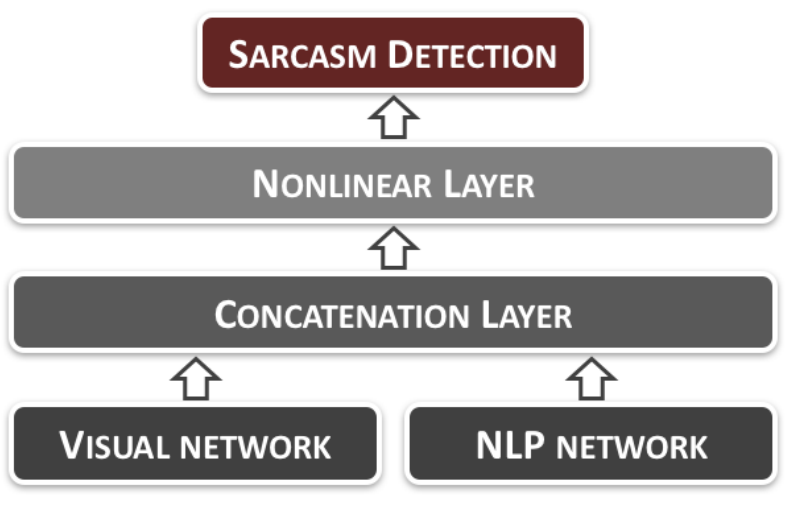
\includegraphics[width=0.85\linewidth]{figures/schifanella2016_architecture.png}
\caption{Neural fusion architecture from Schifanella et al.~\cite{schifanella2016}, original Fig.~3. Text and image networks feed a concatenation layer.}
\label{fig:schifanella}
\end{figure}

The human study shows that images can change sarcasm judgments. Automatic gains are less consistent. On the Twitter silver set, the strongest combined text features reach 80.5\% accuracy. Adding visual concepts gives 80.0\%. Images can help, but simply adding them does not guarantee better predictions.

\subsubsection{A Deeper Look into Sarcastic Tweets Using Deep Convolutional Neural Networks}
Poria et al.~\cite{poria2016} predict sarcasm from text only. The researchers choose sentiment, emotion, and personality as supporting tasks before training. These tasks are fixed design choices, not categories discovered by the model. Figure~\ref{fig:poria} shows how their features are combined.

The CNNs first learn from separate labeled datasets:
\begin{itemize}
\item The sentiment CNN uses SemEval 2014 tweets labeled positive, negative, or neutral.
\item The emotion CNN uses blog sentences labeled with six emotions: anger, disgust, surprise, sadness, joy, and fear.
\item Five personality CNNs use labeled essays. Each predicts the presence or absence of one trait: openness, conscientiousness, extraversion, agreeableness, or neuroticism.
\item A separate sarcasm CNN learns directly from tweets labeled sarcastic or not sarcastic.
\end{itemize}

The trained networks then process the same tweets from the sarcasm dataset. Their hidden layers provide feature vectors, rather than only predicted task labels. These vectors are combined to train the final sarcasm classifier, using an SVM or a neural classifier. The sarcasm tweets therefore need only sarcasm labels. They do not require sentiment, emotion, or personality annotations. The auxiliary datasets supply that supervision during the earlier training stage.

\begin{figure*}[t]
\centering
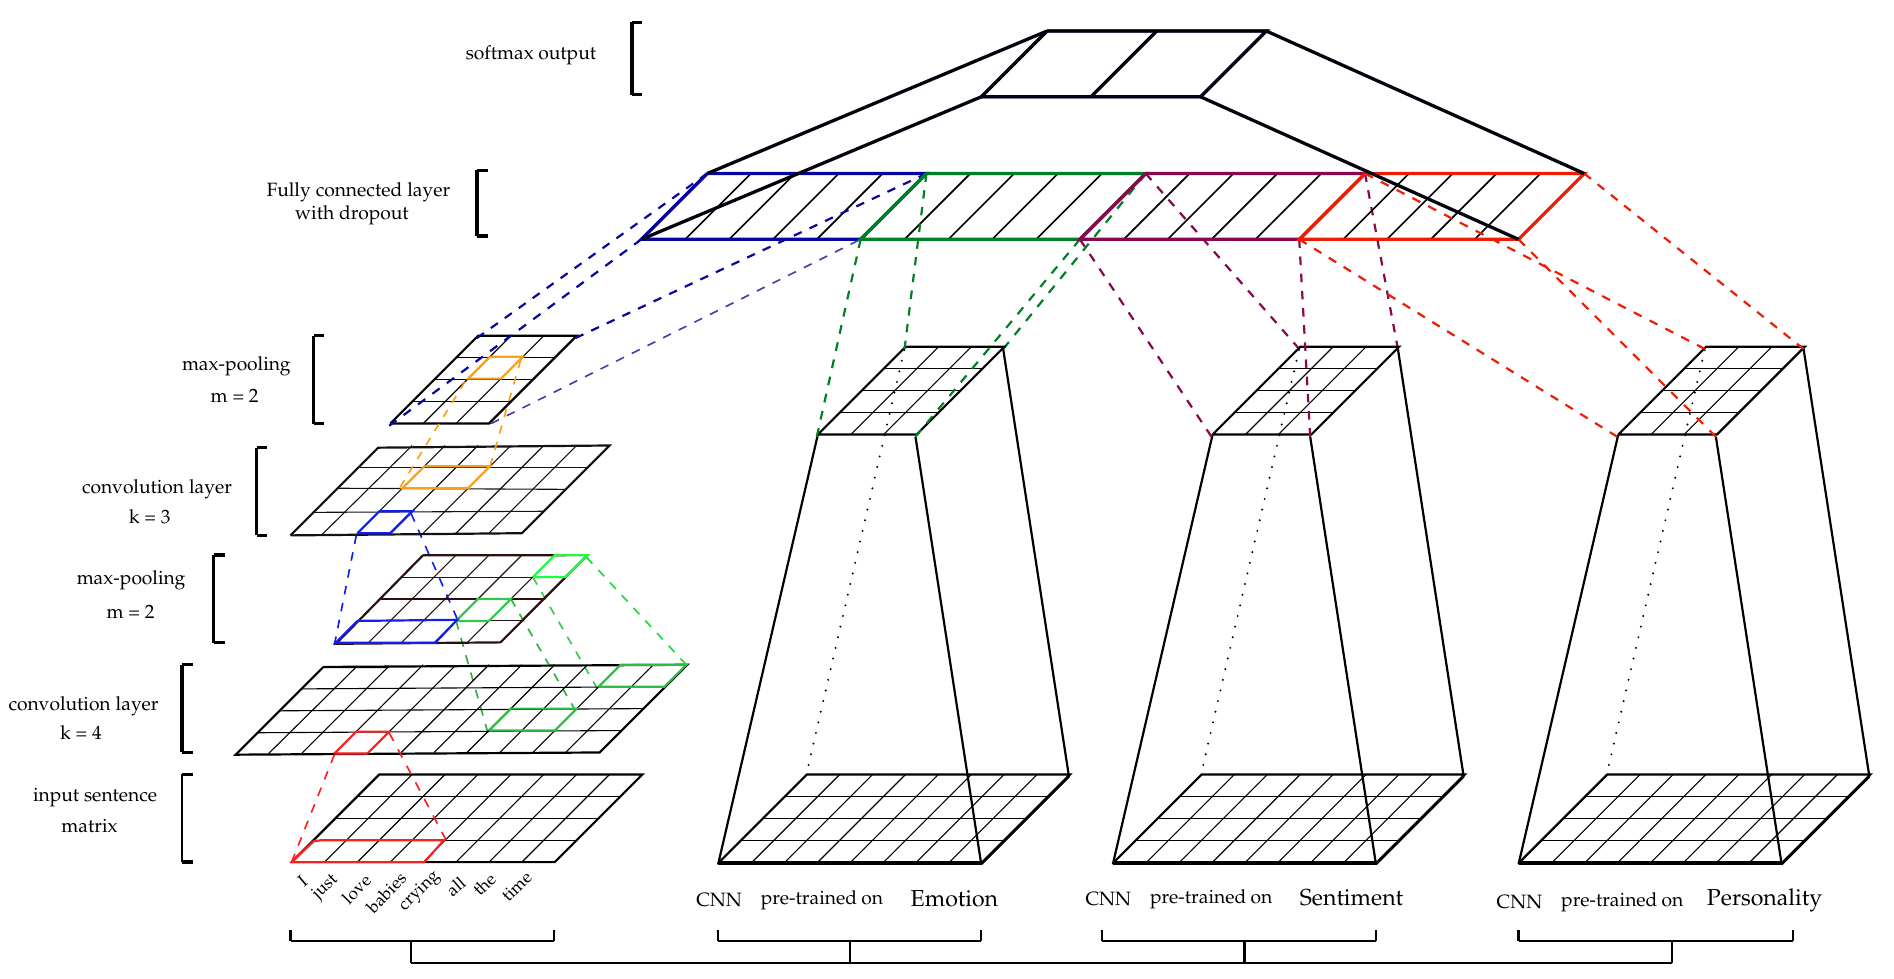
\includegraphics[width=0.80\textwidth]{figures/poria2016_architecture.png}
\caption{Combined CNN architecture from Poria et al.~\cite{poria2016}, original Fig.~2. CNNs trained on separate tasks extract features from the same tweet for sarcasm classification. The personality branch represents five binary CNNs, one per trait.}
\label{fig:poria}
\end{figure*}

The main idea is to transfer knowledge about affect and personality into sarcasm detection. These are different views of the text, not additional observed modalities. The authors compare feature combinations and report macro-F1 on several Twitter datasets. Their F1 falls to 33.05\% when training on Dataset~1 and testing on Dataset~3. Strong results within one dataset therefore do not ensure transfer to another. This motivates a strong language baseline, although our Bi-LSTM does not reproduce their full system.

\subsubsection{Multi-Modal Sarcasm Detection in Twitter with Hierarchical Fusion Model}
Cai et al.~\cite{cai2019} introduce MMSD and combine three representations (Fig.~\ref{fig:cai}). A ResNet produces image region features. A separate predictor supplies five image attributes, which are embedded as words. A bidirectional LSTM encodes the tweet.

We select this paper for reproduction because its staged fusion can be compared directly with feature concatenation. Section~\ref{sec:technical} explains the selected method in detail.

\begin{figure*}[t]
\centering
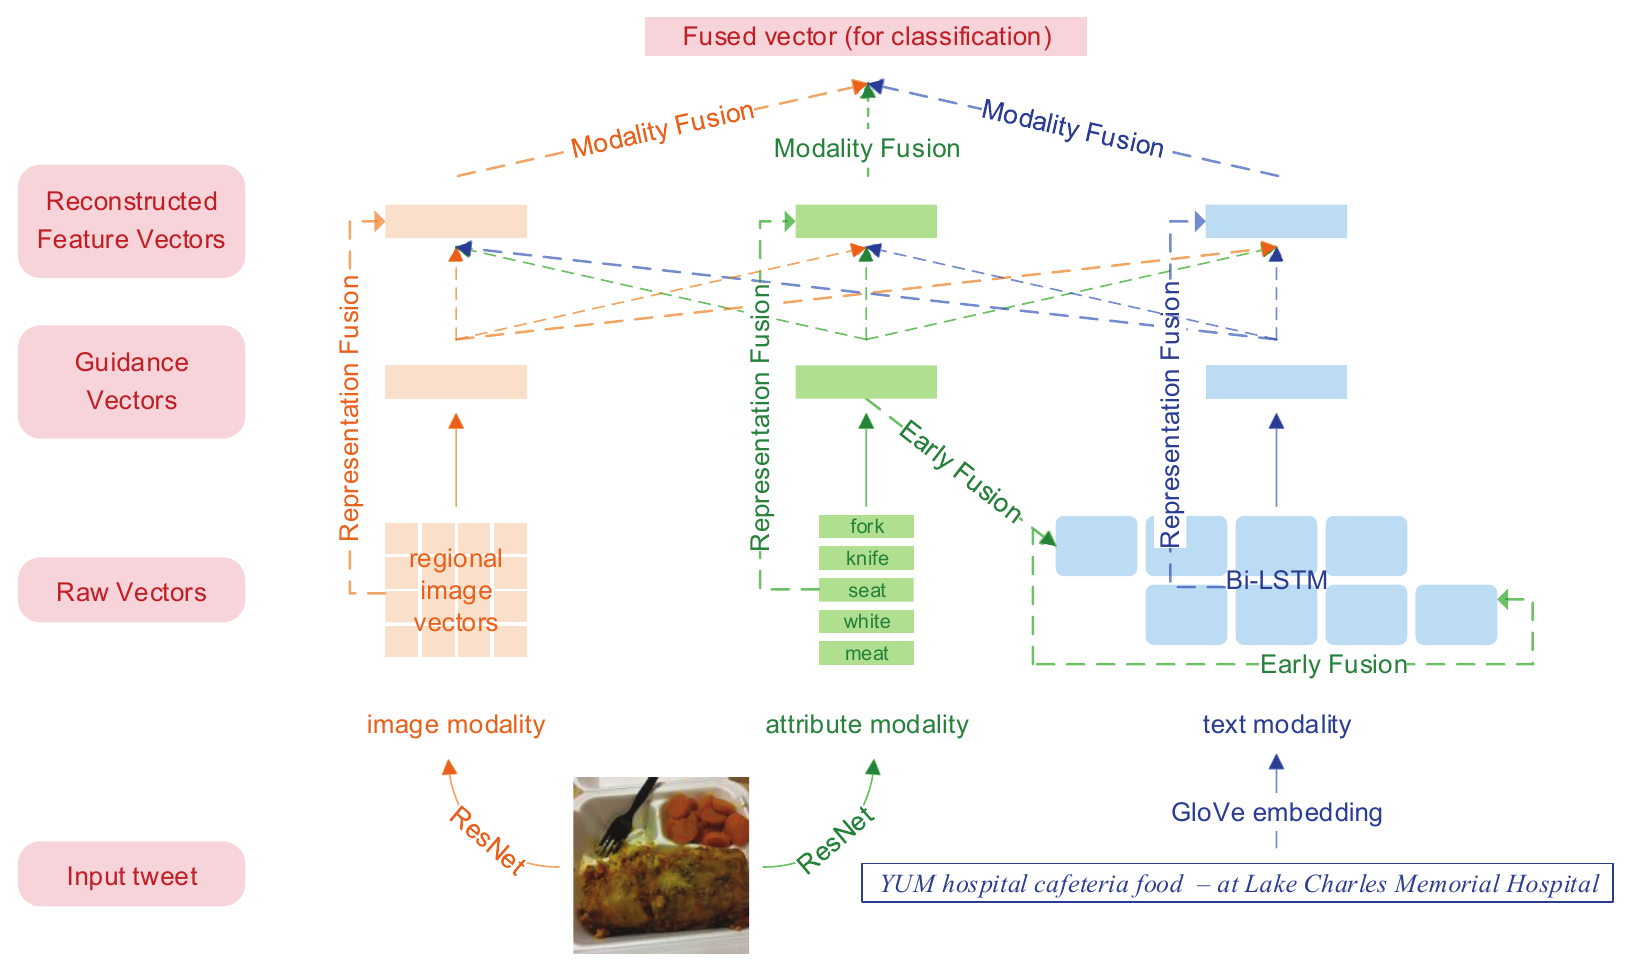
\includegraphics[width=0.82\textwidth]{figures/cai2019_architecture.png}
\caption{Hierarchical fusion architecture from Cai et al.~\cite{cai2019}, original Fig.~2. Early fusion, representation fusion, and modality fusion connect text, image regions, and image attributes.}
\label{fig:cai}
\end{figure*}

Fusion has three stages. First, the attribute representation initializes the LSTM states. The image can therefore influence how the text is encoded. Second, guidance from each representation determines attention over words, image regions, and attributes. Weighted sums produce refined vectors. Third, the model learns how much weight to assign to each vector before classification. Sarcasm labels train the classifier and fusion layers through cross-entropy.

The authors report 80.18\% positive-class F1, compared with 78.74\% for concatenation. Removing the first or second fusion stage lowers F1 to 78.80\% or 79.02\%. These controls support staged interaction in their setting. They do not establish the same gain with different image features or attribute predictors.

\subsubsection{Dynamic Routing Transformer Network for Multimodal Sarcasm Detection}
Tian et al.~\cite{tian2023} propose DynRT-Net (Fig.~\ref{fig:tian}). RoBERTa encodes text tokens, and a vision transformer (ViT) encodes image patches. Cross-attention lets each text token use information from the image patches. An attention mask controls which patches are available. One mask allows access to the whole image. Others restrict access to spatial neighborhoods of different sizes.

Dynamic routing learns how to weight these mask patterns for each input image. At each layer, the router averages the image patch features and passes the result through a small neural network. Its output assigns weights to the available masks. The weighted masks then control attention between text and image features. Routing therefore changes where the text can gather visual information. It is not a choice between separate sarcasm classifiers.

The hierarchy expands the available patterns across layers. The four layers offer one, two, three, and four mask options, respectively. Later layers can combine more spatial scales. Text features are updated through this attention, followed by text self-attention and a feed-forward network. The router and attention parameters learn from the final sarcasm classification loss. No routing labels are required.

\begin{figure*}[t]
\centering
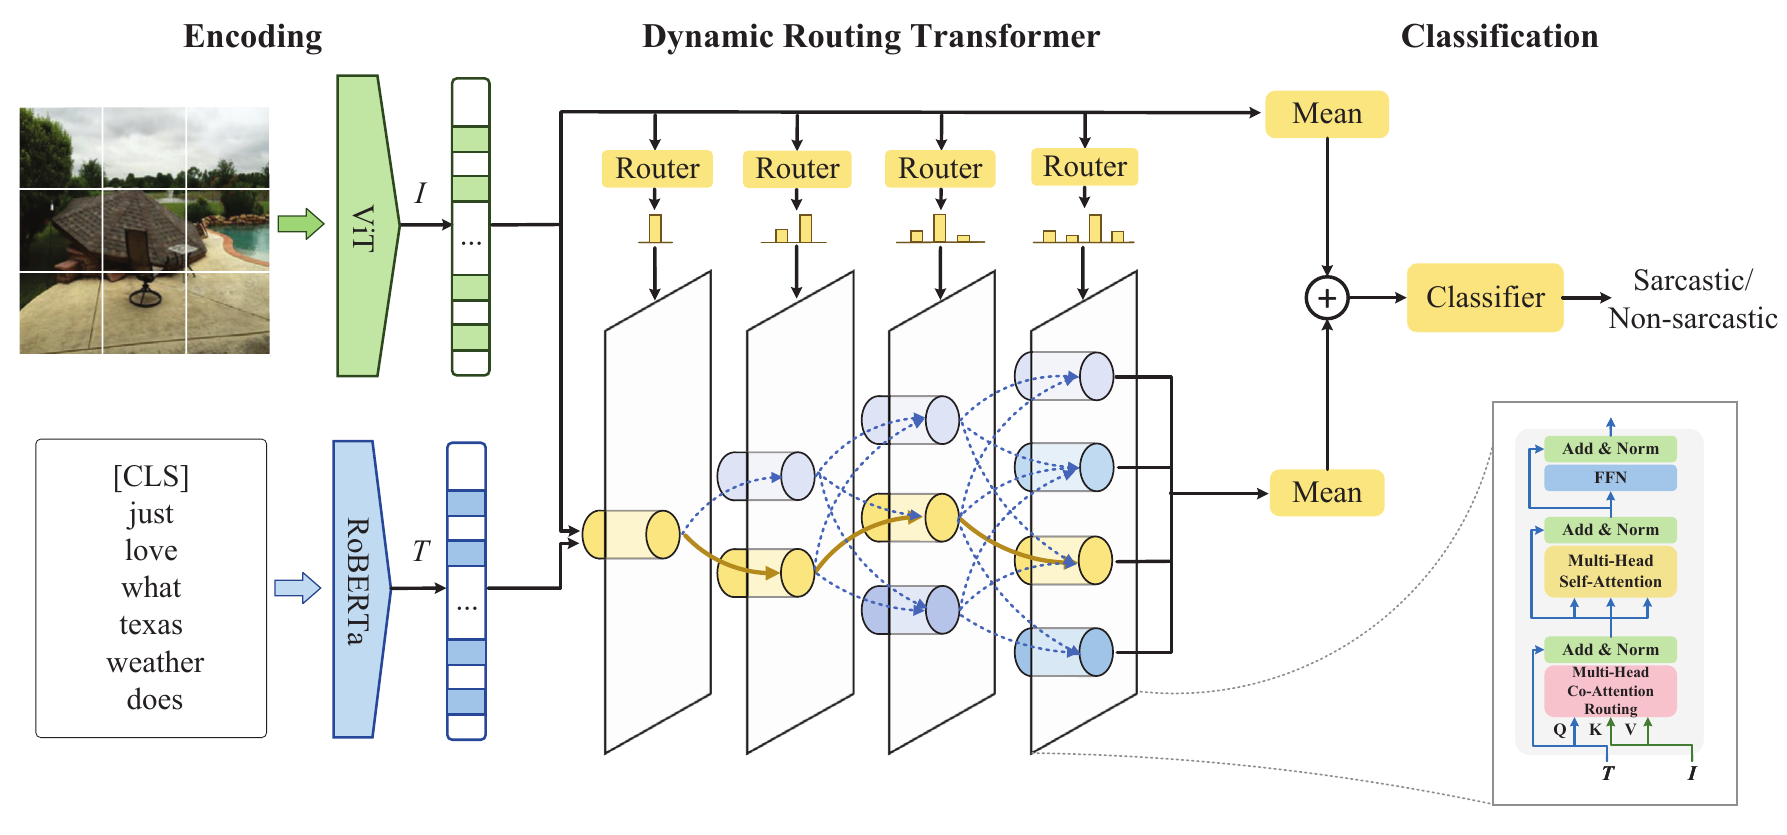
\includegraphics[width=0.90\textwidth]{figures/tian2023_architecture.png}
\caption{DynRT-Net architecture from Tian et al.~\cite{tian2023}, original Fig.~2. Each router uses image features to weight spatial masks. These masks control attention from text tokens to image patches. Later layers offer more mask options.}
\label{fig:tian}
\end{figure*}

The final text and image features are pooled and combined for classification. Cross-entropy trains the model. The authors report 93.21\% macro-F1 and 93.49\% accuracy. Replacing dynamic attention with fixed or mean attention reduces their scores. This supports adaptive interaction in their setup. However, the stronger encoders and different F1 definition prevent a direct comparison with HFM's published score.

\subsubsection{Debiasing Multimodal Sarcasm Detection with Contrastive Learning}
Jia et al.~\cite{jia2024} propose DMSD-CL to reduce reliance on words that happen to correlate with sarcasm labels. RoBERTa and ViT encode the inputs. Cross-attention lets image features attend to text features before classification.

The main contribution concerns training rather than a new fusion architecture. The authors create revised texts while keeping the image. Some revisions change the sarcasm label with minimal wording changes. Others preserve the label while changing the wording. A contrastive loss pulls representations with the same label closer and separates those with different labels. Adaptive weights emphasize pairs that are difficult because of their wording. This loss is combined with the classification loss.

The authors also construct a test set of 400 manually revised examples. It changes the usual association between words and labels. DMSD-CL reaches 67.03\% positive-class F1 on this set. Removing contrastive learning lowers it to 15.38\%. The result supports their training strategy on this controlled shift. It does not establish robustness to every kind of new social media content.

\subsection{Comparison Matrix}
Table~\ref{tab:literature} compares the methods, data, evidence, and reproducibility. Figures~\ref{fig:schifanella} through~\ref{fig:tian} reproduce architectures from the source papers. Resource details also come from the papers. Their released systems were not independently rerun for this review.

\begin{table*}[t]
\caption{Comparison of the five selected papers. Details describe the source studies, not local experiments.}
\label{tab:literature}
\centering
\scriptsize
\setlength{\tabcolsep}{2pt}
\renewcommand{\arraystretch}{1.15}
\begin{tabular}{|P{0.065\textwidth}|P{0.11\textwidth}|P{0.11\textwidth}|P{0.135\textwidth}|P{0.115\textwidth}|P{0.125\textwidth}|P{0.115\textwidth}|P{0.13\textwidth}|}
\hline
\textbf{Paper} & \textbf{Question / contribution} & \textbf{Modalities / assumptions} & \textbf{Mechanism / objective} & \textbf{Data / protocol} & \textbf{Baselines / evidence} & \textbf{Resources / reproducibility} & \textbf{Limitations / connections} \\
\hline
Schifanella et al.~\cite{schifanella2016} & Tests whether images help human and automatic sarcasm detection. & Text and image at inference; noisy hashtag supervision versus reader judgments. & Text and visual-concept concatenation with linear SVM; neural adaptation with a softmax classifier. & Balanced silver sets: 20K each for Instagram/Tumblr, 4,050 Twitter; 50/50 train/test; curated gold subsets. & Text/image/fusion controls; Twitter SVM fusion does not beat strongest text features. & Feature recipes, pretrained CNN source, and neural schedule supplied; checkpoint/hardware provenance not established here. & Small curated subsets; label subjectivity; motivates a strong concatenation control. \\
\hline
Poria et al.~\cite{poria2016} & Transfers sentiment, emotion, and personality knowledge. & Text at inference; auxiliary labeled corpora for pretraining. & Separate CNN feature extractors; combined vectors with SVM or neural classification. & 100K balanced and 100K imbalanced tweets; 30K third corpus subset; cross-validation and transfer tests. & Feature combinations and classifier comparisons; large transfer degradation. & Architecture and auxiliary corpora described; environment and checkpoints not verified here. & Text only; motivates a stronger language baseline. \\
\hline
Cai et al.~\cite{cai2019} & Introduces MMSD and staged fusion. & Text, regions, five predicted attributes; paired inputs required. & Attributes initialize Bi-LSTM; guided attention refines vectors; learned weights fuse them; cross-entropy. & 19,816/2,410/2,409 examples; cue filtering; manually checked dev/test labels. & Unimodal and concatenation controls; stage ablations; paired sign tests. & Assets and hyperparameters available; visual extraction and checkpoint details incomplete. & Sensitive to attribute quality; central reproduction target. \\
\hline
Tian et al.~\cite{tian2023} & Adapts interaction paths to each pair. & Paired text/image; RoBERTa and ViT pretraining. & Router selects attention patterns; hierarchical co-attention; cross-entropy. & MMSD with 19,816/2,410/2,409 split; macro-F1 and accuracy. & Routing and attention replacements; selected shared encoder controls; some imported scores. & Code linked; RTX 2080 Ti, 15 epochs, batch 32; about 238M parameters and 40 min training reported. & Stronger encoders complicate HFM comparison; F1 definitions differ. \\
\hline
Jia et al.~\cite{jia2024} & Reduces spurious textual correlations rather than only improving IID scores. & Text/image at inference; ChatGPT augmentation and entity tools during preparation. & RoBERTa/ViT cross-attention; classification plus adaptive contrastive loss. & MMSD; paper lists 19,815 training examples; standard test plus 400 manually revised OOD cases. & Modality, adaptive-weighting, and contrastive ablations; IID/OOD comparison. & Code/data release stated; backbone, optimizer, augmentation, and loss settings given; hardware not established here. & Generated-label fidelity and curated OOD scope; motivates bias-aware evaluation. \\
\hline
\end{tabular}
\end{table*}

\subsection{Synthesis and Research Gap}
The papers address three questions. Does the image add useful information? How should the inputs interact? Does the model learn sarcasm rather than dataset shortcuts?

Schifanella et al. motivate using images but show that concatenation gains can be small. Poria et al. motivate stronger text features and transfer tests. Cai et al. introduce explicit interaction between representations. Tian et al. make that interaction adaptive. Jia et al. change training to discourage shortcuts.

This project focuses on an input-quality question left open by the staged-fusion design: what happens when the words used to describe the image change? HFM can propagate an incorrect attribute into text initialization, reconstruction attention, and final fusion. A richer attribute predictor might help without redesigning all three stages. CLIP~\cite{radford2021} supplies the enabling representation: its contrastive pretraining aligns image and text embeddings, allowing images to be scored against natural-language prompts. It is used here as a frozen feature-preparation model, not as a sarcasm classifier. This is a focused extension of HFM, not a claim that generic image--text alignment solves sarcastic incongruity.

\section{Technical Explanation of the Selected Method}
\label{sec:technical}
\subsection{Overview}
The selected model predicts whether a tweet is sarcastic by reading its text together with its image. Figure~\ref{fig:cai} shows the architecture proposed by Cai et al.~\cite{cai2019}. It uses three representations: tweet words, image regions, and predicted image attributes. Fusion occurs at three stages. Attributes first guide text encoding. Attention then refines each representation. Finally, learned weights combine the three representations for classification.

The model keeps both detailed features and a summary of each representation. Detailed features describe individual words, regions, or attributes. The summaries are called \emph{guidance vectors}. They provide context when the model decides which detailed features to emphasize.

\subsection{Representing the Image}
A pretrained ResNet-50 V2 converts the image into numerical features. These describe visual patterns rather than directly predicting sarcasm. Keeping features from different spatial locations preserves more detail than reducing the whole image to one vector immediately.

The paper resizes images to 448 by 448 pixels and describes 196 region representations arranged in a grid of 14 by 14 locations. Averaging the region vectors produces the image guidance vector. The individual region vectors remain available for later attention. This gives the model both a summary of the image and access to more detailed visual information.

\subsection{Predicting and Representing Image Attributes}
A separate ResNet-101 predicts words associated with the image. It is trained beforehand using COCO images and their captions. The captions supply a vocabulary of 1,000 candidate attributes. An image can have several attribute labels, so this is a multilabel prediction task. For each tweet image, the predictor returns its five highest scoring words. The candidates are fixed during predictor training, but the selected five words depend on the image.

These attributes describe visual content, such as objects, actions, or appearance. They are not sentiment or personality categories. They give the model a language-based description of the image. This can help connect visual information with tweet words. However, they are predicted descriptions, not verified facts about the image.

Each predicted word is converted into a GloVe embedding with 200 values. A small attention network assigns a score to each of the five embeddings. The scores are normalized into weights that sum to one. Their weighted average becomes the attribute guidance vector. This lets the model emphasize some predicted words more than others. All five embeddings are retained for later fusion.

\subsection{Early Fusion: Letting Attributes Guide Text Encoding}
Tweet words are also converted into GloVe embeddings. A bidirectional LSTM reads the sequence in both directions. This allows each word representation to include context from the words before and after it.

A conventional text encoder can begin with empty internal states. HFM instead transforms the attribute guidance vector into the LSTM's starting hidden and memory states. This gives the text encoder information about the image before it reads the tweet. It is called early fusion because the interaction happens while the text representation is being formed, not only after text encoding is complete.

For example, attributes describing clouds and rain could provide context for the phrase ``wonderful weather.'' This is an illustration of the intended mechanism, not a claim that the model explicitly reasons about weather. Incorrect attributes can also provide misleading context.

The LSTM produces one feature vector for each word by combining its forward and backward hidden states. Averaging these word vectors produces the text guidance vector. The individual word vectors remain available for later attention, just as the region vectors do for the image.

\subsection{Representation Fusion: Selecting Relevant Details}
At this point, the model has detailed features and guidance vectors for text, image, and attributes. Representation fusion uses all three guidance vectors to decide which details matter within each representation.

Consider the image regions. One attention network scores the regions using text guidance. Another uses attribute guidance. A third uses image guidance. Each produces a set of weights across the 196 regions. Each set sums to one. The model averages the three sets of weights and uses the result to combine the region vectors into one refined image vector.

The same procedure is applied to the tweet words and the five attribute embeddings. There are therefore nine guided attention operations: three guidance sources for each of three target representations.

The output is three refined vectors, one for text, one for the image, and one for attributes. Each has been formed using context from all three sources, including its own summary. Attention changes how strongly features contribute. It does not add missing visual knowledge or guarantee that the selected details explain sarcasm correctly.

\subsection{Modality Fusion: Combining the Refined Vectors}
The three refined vectors have different sizes. Separate learned layers map them into a common space with 512 values each. Another set of small networks assigns an importance score to each representation. The three scores are normalized into weights that sum to one. The weighted vectors are then added to form a single fused vector.

These weights depend on the input. They are not fixed percentages chosen before training. The model can give more weight to text for one tweet and more weight to visual information for another. This differs from concatenation, which joins the vectors into a longer vector without this explicit weighting step.

\subsection{Classification and Learning}
A small neural classifier converts the fused vector into a probability of sarcasm. It has one hidden layer and one output. During training, this probability is compared with the tweet's sarcasm label using cross-entropy. Confident wrong predictions receive a larger penalty.

The classification error updates the word and attribute embeddings, text encoder, attention networks, fusion layers, and classifier. Separate attention labels or modality importance labels are not needed. The visual encoders are prepared beforehand and remain fixed during this task training. Their region features and predicted attribute words serve as inputs.

The central idea is therefore repeated interaction, not simply adding more features. Attributes influence text encoding first. Guidance then determines which details enter each refined vector. Learned modality weights finally determine how those vectors contribute to the decision.

\section{Reproduction Target, Implementation, and Deviations}
\label{sec:reproduction}
\subsection{Testable Target}
The source-paper claim is that hierarchical interaction improves over concatenation of the same three representation types. The expected observation is a positive F1 difference between HFM and a three-way concatenation control using the same image features, attribute predictions, data, training budget, and seed set. An advantage that disappears across seeds, changes sign, or vanishes after correcting padding would weaken the claim under this reproduction setting. Matching the paper's rounded absolute score alone would not reproduce its comparative result.

\subsection{Implementation and Artifact Mapping}
The repository contains separate notebooks and result directories rather than one packaged training application. The relevant completed experiment families are:
\begin{itemize}
\item \texttt{text\_only/}: text-only Bi-LSTM; the notebook filename \texttt{fusion-full.ipynb} does not describe its actual text-only model.
\item \texttt{concat2/}: text--image concatenation using fine-tuned regional features, without attributes.
\item \texttt{concat3\_base\_model/}: three-way concatenation using ImageNet-only ResNet-50 V2 features and locally predicted COCO attributes.
\item \texttt{concat3\_paper/}: concatenation using task-fine-tuned visual features and the same attribute prediction path. Despite its notebook filename, the current code uses packed recurrence and masked mean pooling.
\item \texttt{fusion\_full/}: hierarchical-fusion outputs with task-fine-tuned visual features and locally predicted attributes.
\item \texttt{fusion\_clip/}: the proposed attribute intervention. Its notebook is \texttt{fusion-clip.ipynb}; results are under \path{results/runs/hierarchical_finetuned_clip_sentiment_packed/} within that directory.
\end{itemize}
Each family has seeds 42, 43, and 44, with configuration, training history, per-seed results, test predictions, and an aggregate summary. The older \texttt{concat3\_result/} directory contains checkpoints only; it is not another model. Visual preparation is implemented in \path{notebooks/train_resnet50v2_image_classifier.ipynb} and \path{notebooks/extract_resnet50v2_image_regions.ipynb}; baseline attribute preparation is in \path{notebooks/train_resnet101_coco_attribute_predictor.ipynb}.

\subsection{Feature Extraction and Sequence Handling}
Our visual extractor processes each resized image in one full forward pass. Its spatial output supplies 196 vectors with 2,048 values each. These are not independently encoded image crops. A trainable projection reduces each vector to 1,024 values during task training. The source paper's regional extraction description does not fully establish this exact procedure.

Our Bi-LSTM has 256 hidden units in each direction, giving 512 values per word. The corrected notebooks exclude padding from recurrence and mean pooling. The hierarchical model also excludes padded positions from reconstruction attention. Empty text sequences are rejected. These choices prevent batch padding from contributing as though it were tweet content. Visual features are cached, and predicted attribute words are loaded before task training.

\subsection{Deviations from the Source}
This is a pipeline-level reproduction, not an exact recovery of the authors' training environment. It uses PyTorch rather than the upstream TensorFlow implementation, a \texttt{timm} ImageNet-1k \texttt{resnetv2\_50.a1h\_in1k} initialization, direct bicubic resizing, and an explicitly chosen image fine-tuning schedule. The original visual checkpoint and extraction procedure are not recovered. The locally trained ResNet-101 replaces the original attribute predictor, while the supplied word and attribute embedding matrices are reused and updated during task training. Unknown attribute words map to the upstream attribute vocabulary's unknown token; this can discard distinctions introduced by the new predictor.

The local attribute notebook lowercases COCO 2017 training captions, extracts alphabetic words with a regular expression, counts each word once per caption, and selects the most frequent 1,000 words. Labels are the union of these words over an image's captions. It makes a seeded 90/10 image-ID split within the COCO training collection, not the official COCO train/validation partition, despite an inaccurate comment in the notebook. ResNet-101 is fine-tuned with multilabel BCE, Adam at $10^{-4}$, batch 64, and eight epochs; validation loss selects its checkpoint. The top five scores become MMSD attributes. The vocabulary is constructed before that internal split, so it also reflects held-out caption word frequencies. These choices should not be presented as recovered settings from Cai et al.

The sarcasm notebooks use a maximum of eight epochs, exponential learning-rate decay, positive-class loss weighting, and validation-F1 checkpoint selection. None of the local measurements should be interpreted as a direct ranking against a source result trained with a different checkpoint, schedule, or objective.

There are also differences inside the trainable model. Attribute attention uses ReLU instead of the paper's hyperbolic tangent activation. The positive-class loss weight is approximately 1.293. L2 regularization uses a coefficient of $10^{-7}$ and covers all trainable parameters except the word embedding matrix. This is broader than the paper's description of classification-layer regularization.

\subsection{Code and Result Provenance}
The experiment author confirms that the retained \texttt{fusion\_full} outputs were regenerated after the padding correction. Both COCO-HFM and CLIP-HFM therefore use packed recurrence, masked text pooling, and masked text reconstruction attention; their saved configurations record these settings. The obsolete baseline notebook warning has been removed. This run-history confirmation is distinct from independently replaying training. The concatenation comparison and filtered-attribute notebooks retain warnings about earlier outputs, and the text notebook warns about earlier root-level outputs. Their comparisons remain subject to those separate provenance limitations. Prediction checks verify metrics, but cannot recover missing historical source commits.

The repository base revision inspected for this report is \texttt{24e508362882} (abbreviated); report edits and some artifacts are additional working-tree changes. This is not a recovered producing revision for historical runs. CLIP's model revision, prompts, candidate vocabulary, preprocessing, and prediction hash are recorded in its extraction manifest. Its visual-feature manifest remains empty, as in the HFM baseline. No claim is made that rerunning corrected notebooks will reproduce all archived numbers exactly.

\section{Proposed Improvement and Rationale}
\label{sec:improvement}
\subsection{Weakness and Hypothesis}
The original attribute predictor learns caption-derived words, chiefly describing objects, scenes, and actions. It has no explicit mechanism for choosing an affective description. Sarcasm may involve a positive statement paired with an unpleasant scene, so descriptive words alone may omit a useful cue. The hypothesis is that \emph{adding an image-grounded affective word to the attribute stream can improve sarcasm classification while retaining descriptive context}. This is a design rationale, not evidence that the selected words accurately measure emotion.

\subsection{Frozen CLIP Attribute Extraction}
We use \texttt{openai/clip-vit-base-patch32} at revision \texttt{3d74acf9a28c6} (full hash in the manifest). The CLIP image and text encoders are frozen. The image processor resizes the shorter side to 224 pixels, center-crops to $224\times224$, and applies the checkpoint's normalization. This is separate from the $448\times448$ ResNet regional-feature path.

The descriptive pool contains 996 words from the supplied attribute vocabulary after excluding a fixed stopword list, the eight affective candidates, and unsupported character patterns. Each word $w$ is encoded with the prompt \texttt{a photo of \{word\}.} For an image $I$ and prompt $p$, the score is cosine similarity,
\begin{equation}
s(I,p)=\frac{f_I(I)^\top f_T(p)}{\lVert f_I(I)\rVert_2\lVert f_T(p)\rVert_2}.
\end{equation}
The five highest-scoring descriptive candidates are retained in order; stable sorting resolves ties. A separate pool uses \texttt{a photo of a scene that feels \{word\}.} with \emph{good, bad, happy, sad, angry, calm, beautiful, ugly}, plus the same prompt with \emph{neutral}. These words include affect and aesthetic judgments; they are not a calibrated sentiment taxonomy.

If neutral has the highest score, including a tie with an affective candidate, the output is the five descriptions. Otherwise, the fifth description is replaced by the highest-scoring affective word. The two pools are ranked separately: there is no cross-pool confidence threshold and no tweet text or sarcasm label is used during extraction. The final input always contains five attribute words (Fig.~\ref{fig:clip}).

\begin{figure*}[t]
\centering
\resizebox{0.98\textwidth}{!}{% Original vector schematic; compiled as part of report.tex.
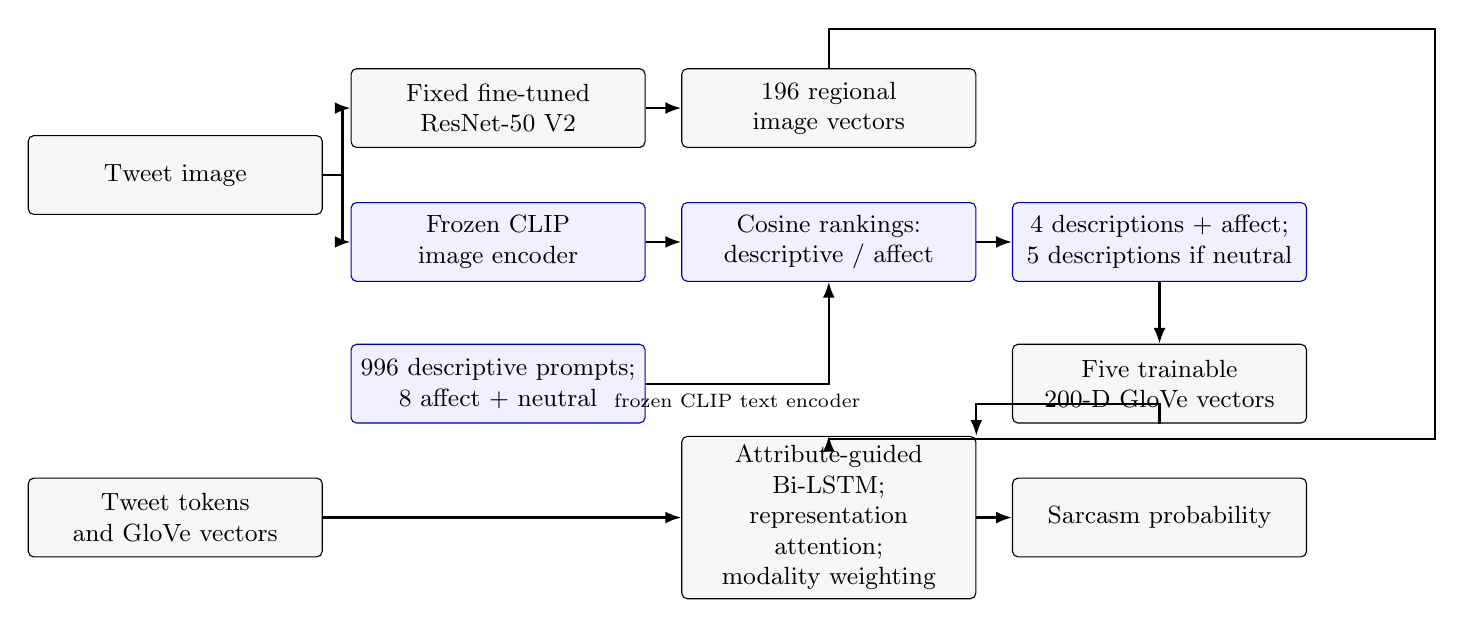
\begin{tikzpicture}[
  box/.style={draw, rounded corners=2pt, align=center, font=\small,
              minimum height=10mm, text width=35mm, fill=black!3},
  changed/.style={box, draw=blue!65!black, fill=blue!6},
  flow/.style={-{Latex[length=2mm]}, thick}]
\node[box] (image) at (0,0) {Tweet image};
\node[box] (resnet) at (4.1,0.85) {Fixed fine-tuned ResNet-50 V2};
\node[changed] (clip) at (4.1,-0.85) {Frozen CLIP\\image encoder};
\node[box] (regions) at (8.3,0.85) {196 regional\\image vectors};
\node[changed] (ranking) at (8.3,-0.85) {Cosine rankings:\\descriptive / affect};
\node[changed] (prompts) at (4.1,-2.65) {996 descriptive prompts;\\8 affect + neutral};
\node[changed] (selection) at (12.5,-0.85) {4 descriptions + affect;\\5 descriptions if neutral};
\node[box] (embed) at (12.5,-2.65) {Five trainable\\200-D GloVe vectors};
\node[box] (tweet) at (0,-4.35) {Tweet tokens\\and GloVe vectors};
\node[box] (fusion) at (8.3,-4.35) {Attribute-guided Bi-LSTM;\\representation attention;\\modality weighting};
\node[box] (output) at (12.5,-4.35) {Sarcasm probability};
\draw[flow] (image.east) -- ++(0.25,0) |- (resnet.west);
\draw[flow] (image.east) -- ++(0.25,0) |- (clip.west);
\draw[flow] (resnet) -- (regions);
\draw[flow] (clip) -- (ranking);
\draw[flow] (prompts.east) -| node[below, pos=0.25, font=\scriptsize] {frozen CLIP text encoder} (ranking.south);
\draw[flow] (ranking) -- (selection);
\draw[flow] (selection) -- (embed);
\draw[flow] (embed.south) |- ([yshift=4mm]fusion.north east) -- (fusion.north east);
\draw[flow] (regions.north) -- ++(0,0.5) -| (16, -3.35) -| (fusion.north);
\draw[flow] (tweet) -- (fusion);
\draw[flow] (fusion) -- (output);
\end{tikzpicture}
}
\caption{Proposed CLIP attribute intervention (original schematic). Blue boxes describe the replacement attribute-preparation path. The regional ResNet path and HFM fusion structure are retained. CLIP scores select words; their numerical scores are not passed to HFM.}
\label{fig:clip}
\end{figure*}

\subsection{Integration and Learning}
Selected words use 200-dimensional GloVe embeddings, not CLIP's dense vectors. Six affective words absent from the attribute vocabulary are initialized from their existing tweet-vocabulary GloVe rows; \emph{happy} and \emph{beautiful} already exist. This expands the matrix from $1002\times200$ to $1008\times200$, adding 1,200 trainable parameters. The matrix remains trainable during sarcasm learning. Attribute attention, attribute-conditioned Bi-LSTM initialization, nine reconstruction attentions, modality weighting, and the classification objective retain the local HFM design.

Image fine-tuning is shared preparation, not the proposed improvement. The local ResNet-50 V2 was adapted using training images and tweet labels with backbone/head learning rates $10^{-5}/10^{-3}$, Adam, batch 32, seed 42, at most eight epochs, and validation-F1 selection. Its head is discarded before frozen regional extraction. The same cached features feed baseline HFM and CLIP-HFM; CLIP replaces only the attribute preparation path, with the vocabulary expansion described above.

\subsection{Control and Possible Failure Modes}
The primary control is local HFM with COCO attributes, using the same recorded split, regional-feature directory, classifier settings, padding treatment, and seed set. This comparison evaluates the entire attribute replacement package: predictor, candidate filtering, prompts, vocabulary extension, and affective selection. It does not isolate sentiment alone. The intended evidence is a repeatable positive F1 difference; a sign change across seeds or a precision--recall trade-off without a clear net gain weakens the hypothesis.

CLIP may assign an aesthetic word to an ordinary scene, miss a small visual detail through center cropping, or replace a useful object description with an irrelevant affective label. Its scores are similarities rather than calibrated probabilities. It is also a much more broadly pretrained model than the baseline predictor. Any benefit cannot automatically be attributed to affect rather than additional pretraining knowledge. These concerns motivate prediction-level inspection and narrow conclusions.

\section{Experimental Design, Data, Metrics, and Resources}
\subsection{Data Version and Preprocessing}
The original MMSD assets are attributed to the authors' repository at upstream revision \texttt{f42b16510208} (abbreviated; full hash in \texttt{data/SOURCE.md}). The local source record lists 24,635 image files. Counting usable examples must nevertheless be based on the text splits and preprocessing, not the number of files in the image directory.

The raw training text file contains 29,040 rows. The notebooks discard any row containing one of the exact whitespace-separated tokens \texttt{sarcasm}, \texttt{sarcastic}, \texttt{reposting}, \texttt{<url>}, \texttt{joke}, \texttt{humour}, \texttt{humor}, \texttt{jokes}, \texttt{irony}, \texttt{ironic}, or \texttt{exgag}. This leaves 19,816 training examples. Validation and test use \texttt{valid2.txt} and \texttt{test2.txt}, taking the final field as the label; filtering leaves their counts unchanged. Table~\ref{tab:data} reports counts recomputed from the local files. This row exclusion is distinct from deleting only the triggering words.

\begin{table}[t]
\caption{Locally audited MMSD splits after notebook cue filtering.}
\label{tab:data}
\centering
\begin{tabular}{lrrr}
\hline
Split & Sarcastic & Non-sarcastic & Total\\
\hline
Training & 8,642 & 11,174 & 19,816\\
Validation & 959 & 1,451 & 2,410\\
Test & 959 & 1,450 & 2,409\\
\hline
\end{tabular}
\end{table}

The notebooks reuse the supplied tokenization and vocabularies rather than retokenizing raw tweets. Sequences are capped at 75 tokens and padded with index zero; no retained example in the audited splits exceeds that cap. Unknown words use the supplied unknown index. The word and attribute matrices have 200 columns. Image features are stored as float32 arrays of shape $196\times2048$; normalization uses the visual checkpoint's configured channel statistics.

\subsection{Split Integrity Audit}
There are no shared tweet IDs between any pair of retained splits. However, comparing the exact stored text strings reveals 31 distinct shared texts between training and validation, 45 between training and test, and eight between validation and test. These are counts of shared unique strings, not counts of all affected rows. Thus, ID-disjoint evaluation is not text-disjoint evaluation. This establishes content overlap, but does not quantify its contribution to F1 or prove image-level duplication. The existing benchmark splits are retained; no deduplication experiment is reported.

\subsection{Baselines and Training Protocol}
The text baseline uses zero-initialized Bi-LSTM states and a mean-pooled text representation. Three-way concatenation combines a 1,024-dimensional pooled image vector, a 512-dimensional text vector, and a 200-dimensional attention-pooled attribute vector, yielding 1,736 features for a $1736\rightarrow256\rightarrow1$ classifier. Concat2 omits the attribute vector. Unlike HFM, these baselines have no attribute-conditioned initial state, guided reconstruction, or modality gate. Concat3 still contains attribute attention, so it is not a completely attention-free control. The ImageNet/fine-tuned Concat3 pair documents a preparatory feature choice rather than the main CLIP intervention.

The recorded common classifier settings are seeds 42, 43, and 44, batch 32, Adam with initial learning rate $0.001$, epoch-wise decay factor 0.8, input dropout 0.2, patience five, gradient clipping at five, and at most eight epochs. The best validation positive-class F1 checkpoint is evaluated on test. Training uses shuffled batches and drops the final incomplete batch; validation and test retain all rows. The classification threshold is strictly $p>0.5$ and is not tuned on test.

The project is exploratory. Saved test scores were inspected across several attribute interventions before CLIP was chosen as the report's focus. Although checkpoint selection uses validation, this is not a preregistered, untouched-test confirmation of the final method. Further CLIP selection-rule experiments were explored on validation; their artifacts were not retained in the final repository, so they are not used as numerical evidence here. A separate retained descriptive-only CLIP control would be needed to attribute a benefit specifically to affective words.

\subsection{Metrics and Uncertainty}
For the sarcastic positive class,
\begin{align}
P&=\frac{TP}{TP+FP},\qquad R=\frac{TP}{TP+FN},\\
F_1&=\frac{2TP}{2TP+FP+FN}.
\end{align}
Accuracy includes both classes. Tables report percentages and, where available, mean $\pm$ sample standard deviation across three seeds ($\mathrm{ddof}=1$), not a confidence interval. The original paper's F-score is positive-class F1, whereas DynRT-Net explicitly reports macro-F1. The two should not be pooled into one leaderboard. A majority-negative classifier has 60.19\% test accuracy but zero positive-class F1.

\subsection{Execution Environment and Resource Accounting}
Saved multimodal configurations record Python 3.13.16, PyTorch 2.11.0 with CUDA 13.0, NumPy 2.1.3, and cuDNN 92700. The saved text runs instead record Python 3.13.18 and CPU-only PyTorch 2.11.0. Concatenation uses one Tesla T4; hierarchical runs list two Tesla T4 devices and use data parallelism when available. CLIP extraction runs on one CUDA device with batch 64; its manifest records Transformers 4.57.1 and Pillow 13.0.0. These are artifact-reported environments, not independently rebuilt historical installations. Fine-tuned run configurations contain empty feature-manifest lists, limiting visual-checkpoint traceability.

Reported task-training times include validation, and test times include loading cached features. They exclude ResNet fine-tuning, COCO attribute training, and feature extraction. CLIP extraction has a separate saved timing and peak-allocation measurement. Peak GPU allocations are PyTorch allocated memory rather than total device consumption. The regional arrays alone require approximately 39.5 GB for 24,635 images, before headers; caching trades storage and loading cost for cheaper task training. CLIP is needed when preparing a new image's attributes, even though it is absent from cached-feature classifier timing.

\subsection{Execution and Reproducibility Boundaries}
The notebooks expect Kaggle-mounted MMSD assets and features. Run the image fine-tuning notebook, then the regional extraction notebook's three parts with its checkpoint. For baseline HFM, train the COCO attribute predictor and use its \texttt{extract\_all}. For the proposed method, \path{fusion_clip/fusion-clip.ipynb} performs CLIP extraction and classifier training; COCO attribute training is not required for this branch, although the supplied attribute vocabulary and GloVe matrix are reused. Set input paths and a fresh output directory before execution. A headless execution command after these path edits is:
\begin{quote}\footnotesize\ttfamily
jupyter nbconvert --to notebook\\
--execute --ExecutePreprocessor.timeout=-1\\
--output-dir=/path/to/executed\\
fusion\_clip/fusion-clip.ipynb
\end{quote}
For the control, substitute \path{fusion_full/fusion-full.ipynb}. These are current execution commands, not recovered historical invocations. The CLIP notebook pins its model revision and Transformers version, refuses to overwrite an existing extraction, and checks manifest hashes before loading words. Its seed runs save configurations, histories, checkpoints, metrics, and predictions. It includes a small synthetic padding check. Running \texttt{python scripts/report\_results.py} independently checks saved predictions and regenerates the report's local result tables without a GPU. \texttt{tectonic report.tex} builds the PDF, including the vector schematic.

The root requirements file does not pin the complete training stack. Exact historical commands, per-run source commits, and the fine-tuned ResNet/COCO checkpoint hashes are not established by the available artifacts. Public data availability is not a redistribution license; access instructions and the upstream revision are recorded in \texttt{data/SOURCE.md}. Thus the tables are reproducible from retained predictions, but full historical training replay is not certified.

\section{Results, Controls, Uncertainty, and Failure Analysis}
\subsection{Original Published Results}
Table~\ref{tab:published} gives source-paper results separately from all repository measurements. The 1.44 percentage-point advantage over three-way concatenation is the comparative target, not an expected exact local score. Cai et al. also report paired sign tests, but not multi-seed variability for these values.

\begin{table}[t]
\caption{Published results from Cai et al.~\cite{cai2019}; not local measurements. All values are percentages.}
\label{tab:published}
\centering
\footnotesize
\begin{tabular}{lrr}
\hline
Model & Positive-class F1 & Accuracy\\
\hline
Text Bi-LSTM & 77.53 & 81.90\\
Text and image concatenation & 77.99 & 81.03\\
Three-way concatenation & 78.74 & 81.74\\
Without early fusion & 78.80 & 82.40\\
Without representation fusion & 79.02 & 82.23\\
Full hierarchical fusion & 80.18 & 83.44\\
\hline
\end{tabular}
\end{table}

\subsection{Completed Local Measurements}
Table~\ref{tab:local} summarizes the six principal experiment families. Across these and the three alternative interventions, all 27 clean test files and six additional corrupted-attribute files were checked. Each contains 2,409 distinct tweet IDs with matching labels across runs. Precision, recall, F1, accuracy, and the strict 0.5 threshold agree with saved metrics; summary means and sample deviations agree with per-seed values. Training histories also agree with saved validation-selected epochs. These checks establish artifact consistency, not producing-code provenance (Section~\ref{sec:reproduction}).

\begin{table*}[t]
\caption{Saved local test measurements, mean $\pm$ sample standard deviation over seeds 42, 43, and 44. All metrics are percentages. COCO-HFM and CLIP-HFM use corrected padding handling. Earlier-baseline provenance limitations are described in Section~\ref{sec:reproduction}.}
\label{tab:local}
\centering
\begin{tabular}{lrrrr}
\toprule
Model & Precision & Recall & F1 & Accuracy \\
\midrule
Text-only & $72.60\pm1.12$ & $85.19\pm1.18$ & $78.38\pm0.36$ & $81.29\pm0.50$ \\
Concat2, fine-tuned & $77.21\pm0.81$ & $82.41\pm1.90$ & $79.72\pm0.90$ & $83.31\pm0.61$ \\
Concat3, ImageNet & $76.96\pm1.90$ & $83.70\pm1.32$ & $80.17\pm0.45$ & $83.51\pm0.70$ \\
Concat3, fine-tuned & $77.98\pm0.74$ & $81.93\pm1.44$ & $79.90\pm0.49$ & $83.59\pm0.30$ \\
HFM, COCO attributes & $76.89\pm0.38$ & $83.73\pm1.47$ & $80.16\pm0.78$ & $83.51\pm0.54$ \\
HFM, CLIP attributes & $76.21\pm1.94$ & $84.98\pm2.08$ & $80.32\pm0.38$ & $83.42\pm0.60$ \\
\bottomrule
\end{tabular}

\end{table*}

The saved ImageNet Concat3 mean exceeds text-only by 1.78 F1 percentage points. Fine-tuned Concat3 is 0.27 points below ImageNet Concat3, and COCO-HFM exceeds fine-tuned Concat3 by only 0.27 points. These comparisons do not reproduce the original 1.44-point matched fusion gain. The local COCO-HFM mean of 80.16\% is close to the published 80.18\%, but matching an absolute score does not recover the authors' relative result or training environment.

\subsection{Effect of the CLIP Intervention}
CLIP-HFM reaches $80.32\pm0.38$\% F1 versus $80.16\pm0.78$\% for COCO-HFM: a difference of \textbf{+0.16 percentage points}. Mean recall rises from 83.73\% to 84.98\%, while precision falls from 76.89\% to 76.21\%. Accuracy decreases by 0.08 percentage points when computed before rounding (83.51\% versus 83.42\% displayed). The change therefore shifts the precision--recall balance rather than improving every quality measure. It is not evidence of a one-point improvement or superiority over the published paper.

\subsection{Seed Variation and Resources}
Table~\ref{tab:seeds} exposes individual F1 values. CLIP's differences from COCO-HFM are +0.45, +0.52, and $-0.48$ points for seeds 42, 43, and 44. The negative third seed weakens a consistent-improvement claim. Its smaller observed sample deviation is not evidence of generally lower variance from only three runs. No significance claim is made. Seeds repeat classifier training; they do not repeat the shared regional or attribute preparation, nor account for dataset sampling uncertainty.

\begin{table}[t]
\caption{Archived positive-class test F1 by seed (\%).}
\label{tab:seeds}
\centering
\small
\begin{tabular}{lrrr}
\toprule
Model & 42 & 43 & 44 \\
\midrule
Text-only & 78.30 & 78.07 & 78.78 \\
Concat2, fine-tuned & 80.06 & 78.70 & 80.40 \\
Concat3, ImageNet & 80.00 & 79.82 & 80.67 \\
Concat3, fine-tuned & 79.38 & 79.96 & 80.35 \\
HFM, COCO attributes & 79.44 & 80.06 & 80.99 \\
HFM, CLIP attributes & 79.88 & 80.58 & 80.51 \\
\bottomrule
\end{tabular}

\end{table}

\begin{table}[t]
\caption{Mean archived task-stage wall time over three seeds. Training includes validation; test includes loading. Preparation costs are excluded.}
\label{tab:resources}
\centering
\small
\begin{tabular}{lrr}
\toprule
Model & Train (s) & Test (s) \\
\midrule
Text only & 600.69 & 1.92 \\
Concat2, fine tuned & 992.22 & 32.64 \\
Concat3, ImageNet & 910.26 & 33.42 \\
Concat3, fine tuned & 1,138.58 & 35.22 \\
HFM, COCO attributes & 1,310.50 & 47.60 \\
HFM, CLIP attributes & 1,211.26 & 33.23 \\
\bottomrule
\end{tabular}

\end{table}

The CLIP classifier has 14,909,926 trainable parameters, including its expanded attribute embeddings; the corresponding local HFM architecture has 14,908,726. CLIP extraction over 24,635 images takes 2,261.73 seconds (37.70 minutes), including model loading, and records 776.67 MiB peak allocated GPU memory. This cost is incurred once for cached attributes, not at each classifier epoch. Mean task-stage training/test times are 1,211.26/33.23 seconds for CLIP-HFM versus 1,310.50/47.60 seconds for COCO-HFM. Text-only ran on CPU, concatenation on one T4, and HFM/CLIP-HFM on two T4s. These are measured run costs, not controlled latency benchmarks: different histories, filesystem caching, and excluded preparation costs prevent a speedup claim. Baseline COCO training cost and comparable HFM task-stage peak memory are unavailable.

\subsection{Other Investigated Attribute Interventions}
Table~\ref{tab:alternatives} retains unfavorable outcomes. Inference-time filtering removes common stopwords from the COCO predictor's ranked classes without retraining it. Whole-attribute dropout zeros all five embedding vectors for 20\% of training examples before attention and all fusion paths. Gated early fusion adds a tweet-conditioned sigmoid scalar that scales the attribute-derived Bi-LSTM hidden and cell initialization, adding 401 parameters. None increases the saved mean clean-input F1 over COCO-HFM. These alternatives address attribute quality or reliance but are not ablations that isolate the sentiment contribution within CLIP.

\begin{table}[t]
\caption{Exploratory alternatives, mean test F1 $\pm$ sample SD (\%). Differences use the saved COCO-HFM baseline. Filtered-attribute outputs retain a separate provenance limitation.}
\label{tab:alternatives}
\centering\footnotesize
\begin{tabular}{lrr}
\toprule
Attribute intervention & Test F1 & $\Delta$ F1 (pp) \\
\midrule
Filtered COCO attributes & $80.01\pm0.80$ & -0.15 \\
Attribute dropout & $79.88\pm0.68$ & -0.29 \\
Gated early fusion & $80.05\pm0.60$ & -0.11 \\
HFM, CLIP attributes & $80.32\pm0.38$ & +0.16 \\
\bottomrule
\end{tabular}

\end{table}

Dropout also yields 79.51\% F1 with missing attributes and 79.59\% with shuffled attributes, versus 79.88\% clean. These are tests of that dropout model only; no corresponding corrupted-baseline result is retained, so robustness improvement is not established. No equivalent robustness claim is made for CLIP.

\subsection{Paired Errors and Illustrative Cases}
Table~\ref{tab:paired} compares per-example predictions against the same labels. At seed 42, CLIP corrects 98 baseline errors but introduces 103. Its confusion counts are $TP=820$, $FP=274$, $TN=1176$, $FN=139$, versus $788,237,1213,171$ for COCO-HFM. More positive detections improve F1 even though five fewer examples are correct overall. This explains why F1 and accuracy can move in opposite directions.

\begin{table}[t]
\caption{CLIP-HFM versus COCO-HFM on identical test IDs. Corrected: baseline wrong, CLIP right; introduced: baseline right, CLIP wrong.}
\label{tab:paired}
\centering\small
\begin{tabular}{rrrr}
\toprule
Seed & Corrected & Introduced & $\Delta$ F1 (pp) \\
\midrule
42 & 98 & 103 & +0.45 \\
43 & 82 & 82 & +0.52 \\
44 & 93 & 94 & -0.48 \\
\bottomrule
\end{tabular}

\end{table}

For transparent case selection, the following are the lowest tweet IDs among seed-42 corrected and introduced errors, respectively. Both images were visually inspected along with the tweet, CLIP attributes, and saved predictions. They illustrate outcomes, not causal explanations of the networks.

\noindent\textbf{Corrected case:} ID \texttt{683295117847969793}, labeled sarcastic, reads ``the pa welcome center is hopping today.'' The image shows a largely empty parking area. CLIP selects \emph{tarmac, parking, runway, sidewalk, ugly}; its sarcasm probability is 0.9754 versus 0.4338 for COCO-HFM. The contrast between ``hopping'' and visible emptiness is consistent with sarcasm. However, \emph{runway} is imprecise and \emph{ugly} is not needed to express that contrast. This example supports neither attribute perfection nor a causal sentiment effect.

\noindent\textbf{Introduced error:} ID \texttt{686667554811691009}, labeled sarcastic, reads ``i bet the guy gets cancer and ends up conquering death in the end \#reusablemovieplots.'' The image is a romantic-style \emph{Deadpool} promotional poster. CLIP selects \emph{room, passengers, touching, gold, beautiful}; its sarcasm probability is 0.4473 versus the baseline's 0.9968. The visual style is captured only loosely, while the film reference and plot-based humor are absent from the five words. Affect alone need not capture cultural knowledge or image text. Neither model's internal reason for the prediction can be established from these outputs.

Across all 24,635 extracted images, neutral wins for 3,320 (13.48\%); an affective word is inserted for the remaining 86.52\%. The word \emph{ugly} alone is selected for 8,052 (32.69\%). This concentration is a diagnostic warning about prompt/candidate bias, not a measured distribution of human sentiment. A nine-prompt argmax is a weak neutrality safeguard when the non-neutral candidates usually win. Attribute validity would require independent annotation or a focused evaluation, not interpreting these selections as ground truth.

\section{Limitations, Conclusions, and Unresolved Questions}
\subsection{Limitations}
The main experimental limitation is effect isolation: the intervention bundles a new predictor, candidate filtering, vocabulary expansion, and sentiment selection. No retained numerical CLIP ablation isolates these factors, so the +0.16-point difference cannot be attributed specifically to sentiment. Deleted exploratory validation outputs are not evidence in this report. Comparing multiple methods after inspecting test scores further limits confirmatory interpretation. The author confirms corrected padding for the principal COCO-HFM comparison, but historical source commits and provenance for some supporting experiments remain incomplete.

Only three classifier seeds are available, with shared feature preparation and no independent replication of pretraining. The fine-tuned visual checkpoint is incompletely traced; end-to-end resource comparison lacks baseline preparation costs. CLIP's much larger external pretraining and possible overlap with web imagery are not controlled. Exact text repetition across splits, noisy hashtag-derived training labels, and untested author/image overlap limit unseen-content claims. The study does not establish missing-input robustness for CLIP, natural-shift performance, or that its selected affective words match human judgments.

\subsection{Conclusions}
HFM provides an explicit mechanism for conditioning language on image attributes, refining representations with guided attention, and learning modality importance. This project reconstructs that pipeline and proposes a focused change: replace supervised COCO attribute prediction with frozen, sentiment-aware CLIP selection while retaining the local fusion structure. This is an implemented attribute-extraction intervention, not a new fusion architecture.

The saved CLIP result is $80.32\pm0.38$\% F1 versus $80.16\pm0.78$\% for local COCO-HFM. Its small positive mean difference accompanies slightly lower accuracy and a negative F1 difference at one seed. The evidence therefore does not establish reliable superiority. The useful outcome is a concrete, reproducible attribute recipe and a bounded evaluation showing both corrections and new failures. The next evidential priorities are a retained descriptive-only CLIP control, independent replication, and duplicate-aware or shifted-data evaluation. These would test whether any gain survives proper isolation rather than continued optimization against the same test set.

\section*{AI Assistance Disclosure}
OpenCode with OpenAI GPT-6 Astra assisted with reading the supplied brief and papers, inspecting notebooks and saved artifacts, experiment-design discussion and notebook preparation, metric and consistency checks, drafting and editing, and the original CLIP pipeline schematic. It also assisted in writing the table-generation script and compiling this IEEE-style \LaTeX{} report. It did not train or rerun the reported models during report preparation. The author remains responsible for the sources, implementation, experimental decisions, and conclusions.

\balance
\begin{thebibliography}{00}
\bibitem{cai2019} Y. Cai, H. Cai, and X. Wan, ``Multi-modal sarcasm detection in Twitter with hierarchical fusion model,'' in \emph{Proc. 57th Annual Meeting of the Association for Computational Linguistics}, 2019, pp. 2506--2515, doi: 10.18653/v1/P19-1239.
\bibitem{schifanella2016} R. Schifanella, P. de Juan, J. Tetreault, and L. Cao, ``Detecting sarcasm in multimodal social platforms,'' in \emph{Proc. ACM International Conference on Multimedia}, 2016, pp. 1136--1145. [Online]. Available: \url{https://arxiv.org/abs/1608.02289}
\bibitem{poria2016} S. Poria, E. Cambria, D. Hazarika, and P. Vij, ``A deeper look into sarcastic tweets using deep convolutional neural networks,'' in \emph{Proc. COLING 2016, the 26th International Conference on Computational Linguistics: Technical Papers}, 2016, pp. 1601--1612. [Online]. Available: \url{https://arxiv.org/abs/1610.08815}
\bibitem{tian2023} Y. Tian, N. Xu, R. Zhang, and W. Mao, ``Dynamic routing transformer network for multimodal sarcasm detection,'' in \emph{Proc. 61st Annual Meeting of the Association for Computational Linguistics}, 2023, pp. 2468--2480, doi: 10.18653/v1/2023.acl-long.139.
\bibitem{jia2024} M. Jia, C. Xie, and L. Jing, ``Debiasing multimodal sarcasm detection with contrastive learning,'' in \emph{Proc. AAAI Conference on Artificial Intelligence}, vol. 38, no. 16, 2024, pp. 18354--18362, doi: 10.1609/aaai.v38i16.29795.
\bibitem{radford2021} A. Radford et al., ``Learning transferable visual models from natural language supervision,'' in \emph{Proc. 38th International Conference on Machine Learning}, PMLR, vol. 139, 2021, pp. 8748--8763. [Online]. Available: \url{https://proceedings.mlr.press/v139/radford21a.html}
\end{thebibliography}

\end{document}
